\documentclass[10pt, a4paper, twocolumn]{article} % 10pt font size (11 and 12 also possible), A4 paper (letterpaper for US letter) and two column layout (remove for one column)

%%%%%%%%%%%%%%%%%%%%%%%%%%%%%%%%%%%%%%%%%
% Wenneker Article
% Structure Specification File
% Version 1.0 (28/2/17)
%
% This file originates from:
% http://www.LaTeXTemplates.com
%
% Authors:
% Frits Wenneker
% Vel (vel@LaTeXTemplates.com)
%
% License:
% CC BY-NC-SA 3.0 (http://creativecommons.org/licenses/by-nc-sa/3.0/)
%
%%%%%%%%%%%%%%%%%%%%%%%%%%%%%%%%%%%%%%%%%

%----------------------------------------------------------------------------------------
%	PACKAGES AND OTHER DOCUMENT CONFIGURATIONS
%----------------------------------------------------------------------------------------

\usepackage[spanish]{babel} % Spanish language hyphenation

\usepackage{microtype} % Better typography

\usepackage{color}

\usepackage{colortbl}

\usepackage{amsmath,amsfonts,amsthm} % Math packages for equations

\usepackage[svgnames]{xcolor} % Enabling colors by their 'svgnames'

\usepackage[hang, small, labelfont=bf, up, textfont=it]{caption} % Custom captions under/above tables and figures

\usepackage{booktabs} % Horizontal rules in tables

\usepackage{lastpage} % Used to determine the number of pages in the document (for "Page X of Total")

\usepackage{hyperref}

\usepackage{graphicx} % Required for adding images

% PONER EL PAQUETE DE HIPERVÍNCULOS

\usepackage{enumitem} % Required for customising lists
\setlist{noitemsep} % Remove spacing between bullet/numbered list elements

\usepackage{sectsty} % Enables custom section titles
\allsectionsfont{\usefont{OT1}{phv}{b}{n}} % Change the font of all section commands (Helvetica)


\usepackage{listings}
%----------------------------------------------------------------------------------------
%	DEFINITIONS
%----------------------------------------------------------------------------------------

\graphicspath{
    {.} % document root dir
    {images/}
}

%----------------------------------------------------------------------------------------
%	XML LISTINGS
%----------------------------------------------------------------------------------------
\definecolor{dkgreen}{rgb}{0,0.6,0}
\definecolor{gray}{rgb}{0.5,0.5,0.5}
\definecolor{mauve}{rgb}{0.58,0,0.82}
\definecolor{gray}{rgb}{0.4,0.4,0.4}
\definecolor{darkblue}{rgb}{0.0,0.0,0.6}
\definecolor{lightblue}{rgb}{0.0,0.0,0.9}
\definecolor{cyan}{rgb}{0.0,0.6,0.6}
\definecolor{darkred}{rgb}{0.6,0.0,0.0}
%	TCL COLORS

\definecolor{TCLmauve}{rgb}{0.58,0,0.82}
\definecolor{TCLblue}{rgb}{0.1176,0.6039,0.8784}
\definecolor{TCLdkgreen}{rgb}{0,0.6,0}

\lstset{
  basicstyle=\ttfamily\footnotesize,
  columns=fullflexible,
  showstringspaces=false,
  numbers=left,                   % where to put the line-numbers
  numberstyle=\tiny\color{gray},  % the style that is used for the line-numbers
  stepnumber=1,
  numbersep=5pt,                  % how far the line-numbers are from the code
  backgroundcolor=\color{white},      % choose the background color. You must add \usepackage{color}
  showspaces=false,               % show spaces adding particular underscores
  showstringspaces=false,         % underline spaces within strings
  showtabs=false,                 % show tabs within strings adding particular underscores
  frame=none,                   % adds a frame around the code
  rulecolor=\color{black},        % if not set, the frame-color may be changed on line-breaks within not-black text (e.g. commens (green here))
  tabsize=2,                      % sets default tabsize to 2 spaces
  captionpos=b,                   % sets the caption-position to bottom
  breaklines=true,                % sets automatic line breaking
  breakatwhitespace=false,        % sets if automatic breaks should only happen at whitespace
  title=\lstname,                   % show the filename of files included with \lstinputlisting;
                                  % also try caption instead of title  
  commentstyle=\color{gray}\upshape
}

\lstdefinelanguage{XML}
{
  morestring=[s][\color{dkgreen}]{'}{'},
  morestring=[s][\color{mauve}]{"}{"},
  morestring=[s][\color{black}]{>}{<},
  morecomment=[s]{<?}{?>},
  morecomment=[s][\color{dkgreen}]{<!--}{-->},
  stringstyle=\color{black},
  identifierstyle=\color{lightblue},
  keywordstyle=\color{red},
  morekeywords={tipo,version,n,pn,icon,help,actualize_tree,v}% list your attributes here
}

\lstdefinelanguage{tcl}
{
  morestring=[s][\color{TCLmauve}]{"}{"},
  morecomment=[l][\color{TCLblue}]{\#},
  morekeywords={set,variable,list,expr,lindex,puts},
  keywordstyle=\color{red},
  stringstyle=\color{TCLdkgreen},
  %morekeywords={tipo}% list your attributes here
}

%----------------------------------------------------------------------------------------
%	MARGINS AND SPACING
%----------------------------------------------------------------------------------------

\usepackage{geometry} % Required for adjusting page dimensions

\geometry{
	top=1cm, % Top margin
	bottom=1.5cm, % Bottom margin
	left=2cm, % Left margin
	right=2cm, % Right margin
	includehead, % Include space for a header
	includefoot, % Include space for a footer
	%showframe, % Uncomment to show how the type block is set on the page
}




\setlength{\columnsep}{7mm} % Column separation width

%----------------------------------------------------------------------------------------
%	FONTS
%----------------------------------------------------------------------------------------

\usepackage[T1]{fontenc} % Output font encoding for international characters
\usepackage[utf8]{inputenc} % Required for inputting international characters

\usepackage{XCharter} % Use the XCharter font

%----------------------------------------------------------------------------------------
%	HEADERS AND FOOTERS
%----------------------------------------------------------------------------------------

\usepackage{fancyhdr} % Needed to define custom headers/footers
\pagestyle{fancy} % Enables the custom headers/footers

\renewcommand{\headrulewidth}{0.0pt} % No header rule
\renewcommand{\footrulewidth}{0.4pt} % Thin footer rule

\renewcommand{\sectionmark}[1]{\markboth{#1}{}} % Removes the section number from the header when \leftmark is used

%\nouppercase\leftmark % Add this to one of the lines below if you want a section title in the header/footer

% Headers
\lhead{} % Left header
\chead{\textit{\thetitle}} % Center header - currently printing the article title
\rhead{} % Right header

% Footers
\lfoot{} % Left footer
\cfoot{} % Center footer
\rfoot{\footnotesize Page \thepage\ of \pageref{LastPage}} % Right footer, "Page 1 of 2"

\fancypagestyle{firstpage}{ % Page style for the first page with the title
	\fancyhf{}
	\renewcommand{\footrulewidth}{0pt} % Suppress footer rule
}

%----------------------------------------------------------------------------------------
%	TITLE SECTION
%----------------------------------------------------------------------------------------

\definecolor{BlueGiD}{cmyk}{0.77,0.17,0.15,0.0}
\definecolor{GrayGiD}{cmyk}{0.82,0.69,0.55,0.59}

\newcommand{\authorstyle}[1]{{\large\usefont{OT1}{phv}{b}{n}\color{GrayGiD}#1}} % Authors style (Helvetica)

\newcommand{\institution}[1]{{\footnotesize\usefont{OT1}{phv}{m}{sl}\color{Black}#1}} % Institutions style (Helvetica)

\usepackage{titling} % Allows custom title configuration

\newcommand{\HorRule}{\color{BlueGiD}\rule{\linewidth}{1pt}} % Defines the gold horizontal rule around the title

\pretitle{
	\vspace{-30pt} % Move the entire title section up
	\HorRule\vspace{10pt} % Horizontal rule before the title
	\fontsize{32}{36}\usefont{OT1}{phv}{b}{n}\selectfont % Helvetica
	\color{GrayGiD} % Text colour for the title and author(s)
}

\posttitle{\par\vskip 15pt} % Whitespace under the title

\preauthor{} % Anything that will appear before \author is printed

\postauthor{ % Anything that will appear after \author is printed
	\vspace{10pt} % Space before the rule
	\par\HorRule % Horizontal rule after the title
	\vspace{20pt} % Space after the title section
}

%----------------------------------------------------------------------------------------
%	ABSTRACT
%----------------------------------------------------------------------------------------

\usepackage{lettrine} % Package to accentuate the first letter of the text (lettrine)
\usepackage{fix-cm}	% Fixes the height of the lettrine

\newcommand{\initial}[1]{ % Defines the command and style for the lettrine
	\lettrine[lines=3,findent=4pt,nindent=0pt]{% Lettrine takes up 3 lines, the text to the right of it is indented 4pt and further indenting of lines 2+ is stopped
		\color{BlueGiD}% Lettrine colour
		{#1}% The letter
	}{}%
}

\usepackage{xstring} % Required for string manipulation

\newcommand{\lettrineabstract}[1]{
	\StrLeft{#1}{1}[\firstletter] % Capture the first letter of the abstract for the lettrine
	\initial{\firstletter}\textbf{\StrGobbleLeft{#1}{1}} % Print the abstract with the first letter as a lettrine and the rest in bold
}

%----------------------------------------------------------------------------------------
%	BIBLIOGRAPHY
%----------------------------------------------------------------------------------------

\usepackage[backend=bibtex,style=authoryear,natbib=true]{biblatex} % Use the bibtex backend with the authoryear citation style (which resembles APA)

\addbibresource{example.bib} % The filename of the bibliography

\usepackage[autostyle=true]{csquotes} % Required to generate language-dependent quotes in the bibliography
 % Specifies the document structure and loads requires packages

%----------------------------------------------------------------------------------------
%	ARTICLE INFORMATION
%----------------------------------------------------------------------------------------

\title{Primer acercamiento al desarrollo de Problem Types en GiD} % The article title

\author{
	\authorstyle{Luis G. Yáñez Rodríguez\textsuperscript{1}} % Authors
	\newline\newline % Space before instittions
	\textsuperscript{1}\institution{Universidad de Guanajuato, Guanajuato, México}\\ % Institution 1
}

% Example of a one line author/institution relationship
%\author{\newauthor{John Marston} \newinstitution{Universidad Nacional Autónoma de México, Mexico City, Mexico}}

\date{Febrero, 2018} % Add a date here if you would like one to appear underneath the title block, use \today for the current date, leave empty for no date

%----------------------------------------------------------------------------------------

\begin{document}

\maketitle % Print the title

\thispagestyle{firstpage} % Apply the page style for the first page (no headers and footers)

%----------------------------------------------------------------------------------------
%	ABSTRACT
%----------------------------------------------------------------------------------------

\lettrineabstract{Sin duda alguna, los modelos computacionales nos han permitido entender el mundo que nos rodea. Ya sea para explicar de una mejor manera un fenómeno o para poder predecirlo. Parte del éxito de estas soluciones tiene que ver con que estas se apoyan de elementos gráficos para la presentación de resultados, en resumen tener algo más o menos ``tangible'', ya que todas las soluciones que en estos métodos se encuentran se resumen en ceros y unos. Existen muchos softwares que ayudan en el pre y post proceso de un método computacional, pero entre ellos destaca uno en particular llamado GiD, The personal pre and post processor, desarrollado por el CIMNE, el cual que permite una amplia adaptación al problema en cuestión y customización de los procesos del modelado matemático.}

\section{Justificación}

Cuando se usa GiD para un análisis en particular, es necesario establecer los parámetros a los que el modelo estará sujeto (preproceso). En esta parte se definen parámetros como, condiciones, materiales, datos generales, sistema de unidades, símbolos y el formato del archivo de salida para el solver\footnote{Conjunto de rutinas de programación para resolver un problema numérico en específico.}. Gracias a la característica de adaptación de \textit{GiD}, los desarrolladores del software crearon una colección de archivos llamada \textbf{Problem Type} que definen los parámetros anteriores. Actualmente la documentación disponible acerca del desarrollo de problem types se encuentra en el idioma inglés, lo cual puede ser una limitante para aquellos que quieran incursionar en el desarrollo de las herramientas. 

\begin{figure}[hbt!]\centering
	
\includegraphics[width=0.2\textwidth]{logoGiD.PNG}
	\caption{Logo de GiD.}
\end{figure}

\subsection{Objetivo}

Este documento pretende ser un ``primer acercamiento'' a los problem types para aquellas personas de habla hispana en donde tal vez no encuentren toda la información, pero sí puedan tener un apoyo.

\subsection{Aplicación}

Cabe señalar que este material será sólo un apoyo para la \textit{customización}, no es un manual de usuario de GiD, este se puede encontrar en \textcolor{BlueGiD}{\underline{\url{www.gidhome.com/support/gid-manuals/}}} . En caso de tener dudas muy puntuales el material de apoyo es muy amplio y siempre se puede consultar el \textit{Manual de Customización} o directamente en los foros de ayuda en donde los desarrolladores de GiD ayudarán, el link es \textcolor{BlueGiD}{\underline{\url{www.gidhome.com/forum/}}}.

\section{Primeros pasos}
\label{sec:manualTCL}
¿Qué es lo que hace interesante GiD?. La respuesta es la \textbf{programación}, GiD está escrito para que sea de propósito general, de manera que los usuarios pueden crear sus propios solvers y manipular la información que sale y entra en él. Para explicar lo anterior, se tiene el siguiente diagrama:

\begin{figure}[hbt!]\centering
	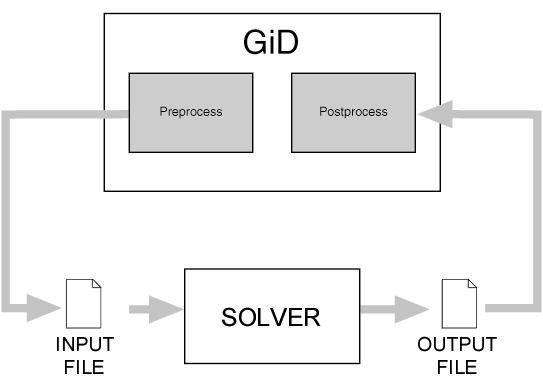
\includegraphics[width=0.35\textwidth]{etapasGiD.PNG}
	\caption{Diagrama de los procesos que realiza un Problem Type.}
	\label{fig:diagramaProcesos}
\end{figure}

La manera como se escribían anteriormente los \textit{problem types} era un poco rudimentaria, de manera que con unas cuantas instrucciones se desplegaban ventanas para la entrada de datos, imposibilitando personalizar estas ventanas.

Desde la versión 13 de GiD, se ha implementado una nueva versión de problem type (basado en la librería CustoLIB), aunque el sistema ``clásico'' sigue siendo soportado por GiD. Esta nueva versión usa un único archivo \texttt{.spd} para describir las propiedades generales, materiales, condiciones y unidades (como un árbol en la sintaxis de \textbf{XML}). Toda esta información se muestra en una ``vista de árbol'' y los materiales y condiciones son asociados en grupos de entidades.

Toda esta información es leída y procesada mediante el lenguaje de programación \textbf{TCL}, lenguaje orientado a objetos que permitirá crear interfaces gráficas de usuario (GUI) y darle un mejor aspecto a los problem types.

La combinación de TCL y XML, definirá el rumbo que el usuario le de a su problem type, es por ello que es importante leer y aprender de estas dos herramientos. Una buena guía para TCL se puede encontrar en: \textcolor{BlueGiD}{\underline{\url{www.tcl.tk/doc/}}}, y para XML en: \textcolor{BlueGiD}{\underline{\url{www.w3schools.com/xml/}}}.

\subsection{El sistema del problem type}

Como ya se dijo, un problem type es una colección de utilidades, las cuales permiten al usuario interactuar fácilmente con ellos mediante una GUI y facilita la definición e introducción de todos los datos necesarios para abordar un cálculo en particular. Para preparar los tos para un programa de análisis específicos, es necesario personalizarlo primero. La personalización se define en GiD por medio de un problem type.

El nuevo sistema para la creación de un problem type agrega algunas capacidades adicionales comparado con el sistema clásico:

\begin{itemize}
	\item Aprovecha las características de formato de XML y su estructura jerarquizada. Almacena información eficientemente. Los elementos en un documento XML forman una estructura de árbol que ``comienza en la raíz y se ramifica en las hojas'' con diferentes relaciones entre los elementos anidados.
	\item Facilita la creación automática de \textit{ventanas estandarizadas} en el árbol de datos (\textit{data tree}) para introducir datos.
	\item Permite acoplar entidades con propiedades idénticas en grupos.
	\item Permite aplicar eficientemente propiedades geométricas y condiciones de contorno en grupos para editar sus propiedades fácilmente.
\end{itemize}

\subsection{Notepad++}
Dada la premisa de que para trabajar en GiD utilizaremos dos lenguajes (XML y TCL), necesitamos una herramienta que nos permita una escritura de código versátil. Existen editores de texto que brindan soporte para los diferentes lenguajes de programación es decir, cuando se crea un archivo con extensión \textbf{\texttt{.cpp}} (C++), \textbf{\texttt{.java}} (Java), \textbf{\texttt{.m}} (MATLAB/Octave), el editor detecta las palabras reservadas del lenguaje en cuestión. Una muy buena opción es \textbf{Notepad++}, un libre editor de código fuente que se puede encontrar en:\\ 

\textcolor{BlueGiD}{\underline{\url{www.notepad-plus-plus.org/download/}}}\\

Cabe mencionar que GiD tiene su editor de TCL incluido (\textit{Data}>\textit{Problem type}>\textit{Debugger...}) sin embargo prefiero usar Notepad++ por su gran eficiencia.

Se utilizará este editor para crear, editar y organizar los archivos que componen el problem type.

\subsection{Mini-tutorial de XML}

\begin{itemize}
	\item ¿QUÉ ES XML?
		\begin{itemize}
			\item XML significa eXtensible Markup Language.
			\item Es un meta-lenguaje que permite representar información estructurada de modo que esta pueda ser almacenada, transmitida, procesada, visualizada e impresa, por diversos dispositivos a través de un \textit{analizador sintáctico}.
		\end{itemize}
	\item ¿QUÉ NO ES XML?
		\begin{itemize}
			\item No es una versión mejorada de HTML.
			\item No es un lenguaje para hacer páginas Web.
			\item No es difícil.
		\end{itemize}
	\item ¿POR QUÉ XML?
		\begin{itemize}
			\item Es un estándar internacionalmente conocido.
			\item No pertenece a ninguna compañía.
		\end{itemize}
\end{itemize}

Este es un ejemplo de cómo luce un XML. Gracias a su característica de marcado, puede ser interpretado por una computadora y por humanos. La primera línea es de carácter obligatorio ya que define los parámetros de lectura del intérprete.

\lstset{language=XML} 
\begin{lstlisting}
<?xml version="1.0" encoding="utf-8"?>
<!-- Esto es un comentario -->
<IntegrantesAulaCIMNEUG>
  <integrante tipo="colaborador">
    <nombre>Luis Guillermo</nombre>
    <grado>Pasante de Ingenieria</grado> 
  </integrante>

  <integrante tipo="responsable">
    <nombre>Humberto Esqueda</nombre>
    <grado>Maestro en Ciencias</grado> 
  </integrante>
</IntegrantesAulaCIMNEUG>
\end{lstlisting}

\subsection{Mini-tutorial de TCL}

\lstset{language=tcl} 

\begin{itemize}
\item Asignar valor a una variable:
\begin{lstlisting}
set entero 1; # Valor entero
set flot 1.0; # Valor flotante 
\end{lstlisting}

\item Asignar valor de una variable a otra:
\begin{lstlisting}
set entero1 "Hola mundo!"; # Uso de cadenas de texto
set entero2 $entero1; # Asignar valor a variable
\end{lstlisting}

\item Operaciones matemáticas:
\begin{lstlisting}
set tres 3.0
set suma [expr 1.0+2.0+$tres]; # Sumar numeros con variables
\end{lstlisting}

\item Crear funciones o procedimientos (\textbf{\texttt{proc}}):
\begin{lstlisting}
proc FuncionSuma { arg1 arg2 } {
	return [expr $arg1+$arg2]; # Regresa suma de dos numeros
}
proc ProgramaPrincipal { } {
	set num1 37.0; # Valor flotante 
	set num2 45.65; # Valor flotante 
	set resultado [FuncionSuma $num1 $num2]; # Se utilizan corchetes para invocar otros programas
	puts $resultado; # Imprimir en pantalla el resultado
}

\end{lstlisting}

\end{itemize}

\subsection{Estructura del problem type}

Un problem type se define creando una carpeta cuyo nombre será el nombre del problem type propiamente, seguido de la extensión ''\textbf{.gid}´´ y en esta se colocarán una serie de archivos que tendrán una estructura específica. Para ejemplificar este \textit{manual} se creará uno llamado \textbf{\texttt{EjemploPT.gid}}.

La carpeta del problem type estará ubicada en el directorio \textbf{problemtypes} de la distribución \textit{GiD} que se tenga instalado en la computadora, por ejemplo en caso que sea la versión \texttt{13.1.0d} en Windows, se debe colocar la carpeta \textbf{\texttt{EjemploPT.gid}} en la dirección:

\begin{verbatim}
	C:\Program Files\GiD\GiD 13.1.0d\problemtypes
\end{verbatim}

Una vez colocada la carpeta en la dirección anterior, crearemos con ayuda de \textbf{Notepad++} y colocaremos en \textbf{\texttt{EjemploPT.gid}} los siguientes archivos:

\begin{table}[hbtp!]
	\label{tab:estructuraArchivos}
	\begin{tabular}{l m{4.5cm}}
		\rowcolor{BlueGiD!60} Nombre del archivo & Descripción\\
		\rowcolor{BlueGiD!20} EjemploPT.spd & Archivo de configuración principal del árbol de datos, basado en \textbf{XML}.\\
		EjemploPT.tcl & Archivo \textbf{TCL} principal, inicialización.\\
		\rowcolor{BlueGiD!20} EjemploPT.cnd & Definición de condiciones. No debería modificarlo el usuario final.\\
		EjemploPT.xml & Define la configuración principal del problemtype.\\
	\end{tabular}
	\caption{Archivos contenidos en \textbf{\texttt{EjemploPT.gid}} para inicializar el problem type.}
\end{table}

De modo que el directorio del problem type se vería así:

\begin{verbatim}
	EjemploPT.gid
	EjemploPT.gid\EjemploPT.spd
	EjemploPT.gid\EjemploPT.tcl
	EjemploPT.gid\EjemploPT.cnd
	EjemploPT.gid\EjemploPT.xml
\end{verbatim}

Teniendo esto, abrimos \textit{GiD}, en el menú \textit{Data}>\textit{Problem type} se debe encontrar el problem type \textbf{\texttt{EjemploPT}}. Si al seleccionarlo no se ha producido ningún error, \textbf{los archivos se han cargado satisfactoriamente}.

\section{Estructura de los archivos}

En esta sección hablaré de la estructura y parámetros de configuración adecuados a los archivos que se describieron en \ref{tab:estructuraArchivos} para comenzar la personalización de GiD.

\subsection{EjemploPT.xml}
\label{sec:codigoXML}
El archivo de configuración inicial XML, contiene datos generales del programa. Este archivo generalmente sólo se configura una sóla vez, ya que los datos sólo son informativos.

Aunque el archivo es muy corto, la información es esencial, no se debe omitir ninguna de estas etiquetas ni modificar los identificadores. Existen más etiquetas para darle más información a GiD sobre nuestro problem type, pero estas son de uso \textbf{obligatorio}.

\lstset{language=XML} 
\begin{lstlisting}
<?xml version="1.0" encoding="utf-8"?>
<Infoproblemtype version="1.0">
  <Program>
    <Name>EjemploPT</Name>
    <Version>1.0</Version>   
    <MinimumGiDVersion>12.1.11d</MinimumGiDVersion>
    <CustomLibAutomatic>1</CustomLibAutomatic>
 </Program>
</Infoproblemtype>
\end{lstlisting}

\textcolor{red}{NOTA:} Cabe señalar que la \textit{etiqueta} \texttt{\textcolor{darkblue}{CustomLibAutomatic}} debe tener el valor de \texttt{\textcolor{darkblue}{1}} (uno). Este activa el uso de la librería \textit{CustomLib} que permite acceder a funciones del nuevo sistema de problem types.
%%%%%%%%%%%%%%%%%%%%%%%%%%%%%%%%%%%%%%%%%%%%%%%%%%%%%%%%%%%%%%
Al escribir esto en el archivo XML, se guardan los cambios en el archivo.

\subsection{EjemploPT\_default.spd}

Este archivo establece la configuración principal del \textit{Árbol de datos} (\textit{Data tree}, en inglés), cuyo fin es estructural las condiciones, materiales y otros datos del modelo computacional.

Como se dijo en \ref{tab:estructuraArchivos}, está basado en XML y los \textit{campos}, \textit{atributos} y otros identificadores que debe contener \textbf{ya están establecidos por GiD} para que el software los interprete y posteriormente crear elementos gráficos con ellos.

% Poner referencia del Customization_Manual.pdf
En XML podemos crear \textit{campos o etiquetas} con cualquier nombre, para almacenar diferentes datos estos identificadores. En la programación de problem types, los nombre de estos campos o etiquetas ya se encuentran reservados y son así para que el GiD pueda interpretarlos y este último pueda crear objetos gráficos. En la documentación de GiD se describe la estructura adecuada para estas \textit{etiquetas}.

Para ramificar el árbol de datos, estas etiquetas pueden anidarse para contener objetos dentro de otros. En este manual solo se describen algunas de ellas:

\subsubsection{$<$PT\_data$>$}

\vspace{0.20cm}
\begin{center}
	\texttt{$<$PT\_data$>$}
\end{center}
\vspace{0.20cm}

Es \textbf{etiqueta principal y obligatoria} del archivo \texttt{.spd}. Contiene el número de versión y el nombre del problem type. Los caracteres \texttt{PT} deben ser remplazados por el nombre del problem type.

\vspace{0.15cm}
\textit{Atributos}:

\vspace{0.15cm}
	\textbf{version} - Número de versión interno.
\vspace{0.15cm}

Como el problem type se llama \texttt{EjemploPT}, el nodo principal es:

\lstset{language=XML} 
\begin{lstlisting}
<?xml version="1.0" encoding="utf-8"?>

<EjemploPT_data version='1.0'>
	...
</EjemploPT_data>
\end{lstlisting}

\subsubsection{$<$container$>$}

\vspace{0.20cm}
\begin{center}
	\texttt{$<$container$>$}
\end{center}
\vspace{0.20cm}


Es la forma más simple de agrupar datos y mejorar su visualización. En la ventana resultante, además de las entradas, se encontrarán los siguientes botones:

\begin{figure}[hbtp!]
	\centering
	
\includegraphics[scale=1]{container.png}
\end{figure}

Puede contener o anidarse en esta etiqueta los siguientes campos: \texttt{<value>}, \texttt{<container>}, \texttt{<condition>}, \texttt{<functions>} y \texttt{<dependencies>} (en este manual no se definirán todas las etiquetas).

\vspace{0.15cm}
\textit{Atributos}:

\vspace{0.15cm}
	\textbf{n} - Nombre usado para referenciar el campo, especialmente cuando se escriben los arhivos \texttt{.dat} y \texttt{.tcl}.\\
	\textbf{pn} - Etiqueta que será visualizada por el usuario.\\
	\textbf{icon} - Permite poner una imagen en formato \texttt{.png} en el \textit{data tree}- La imagen debe ser guardada dentro de la carpeta llamada \texttt{images} del problem type.\\
	\textbf{help} - Despliega una ventana \textit{pop-up} con información de ayuda relacionada a la tarea que el usuario desea realizar. Aparece a los pocos segundos de posicionar el cursor en el container.\\
	\textbf{actualize\_tree} - Actualiza la información que contiene en todo el \textit{data tree} y automáticamente actualiza los datos mostrados en la interfaz del usuario. Es un valor booleano de 1 o 0 indicado si está activada o desactivada esta función.
\vspace{0.15cm}

\textit{Uso}:
\vspace{0.15cm}

\lstset{language=XML} 
\begin{lstlisting}
<?xml version="1.0" encoding="utf-8"?>

<EjemploPT_data version="1.0">
	<container n="contenedor1" pn="Container 1" help="Esto es un ejemplo." actualize_tree="1">
		<container n="contenedor2" pn="Container 2" help="Containers anidados" actualize_tree="1">
			<value n="valor" pn="Valor" v="1.0"/>
		</container>
	</container>
</EjemploPT_data>
\end{lstlisting}

\subsubsection{$<$value$>$}
\label{subsubsec:value}
\vspace{0.20cm}
\begin{center}
	\texttt{$<$value$>$}
\end{center}
\vspace{0.20cm}

Es el campo principal para almacenar datos. Este campo permite definir una \textit{caja de entrada} en la ventana.

\vspace{0.15cm}
\textit{Atributos}:

\vspace{0.15cm}
	\textbf{n} - Nombre usado para referenciar el campo, especialmente cuando se escriben los arhivos \texttt{.dat} y \texttt{.tcl}.\\
	\textbf{pn} - Etiqueta que será visualizada por el usuario.\\
	\textbf{v} - El valor o valor por defecto del campo.\\
	\textbf{values} - Lista de cadenas de caracteres separados por comas. Crea una lista desplegable. Por ejemplo: \texttt{values="Poisson,Young"}.\\
	\textbf{actualize\_tree} - Actualiza la información que contiene en todo el \textit{data tree}.
\vspace{0.15cm}

\textit{Uso}:
\vspace{0.15cm}

\lstset{language=XML} 
\begin{lstlisting}
<?xml version="1.0" encoding="utf-8"?>
<container n="caja" pn="Caja">
  <value n="base" pn="Base:" v="5.00"/>
  <value n="altura" pn="Altura:" v="6.00"/>
</container>
\end{lstlisting}

\textit{Anidar} las etiquetas \texttt{$<$value$>$} en \texttt{$<$container$>$}, como el ejemplo anterior produce lo siguiente:

\begin{figure}[hbtp!]
	\centering
	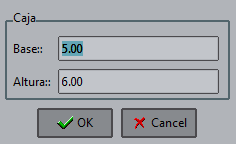
\includegraphics[scale=.8]{value_field.png}
\end{figure}


\subsubsection{$<$blockdata$>$}

\vspace{0.20cm}
\begin{center}
	\texttt{$<$blockdata$>$}
\end{center}
\vspace{0.20cm}

Representa un arreglo de propiedades con algún tipo de relación. Un campo ``\texttt{blockdata}'' puede copiarse a sí mismo para duplicar y crear diferentes arreglos. Esta etiqueta es comúnmente utilizada para uso como \textit{base de datos} del problem type.

\vspace{0.15cm}
\textit{Atributos}:

\vspace{0.15cm}
	\textbf{n} - Nombre usado para referenciar el campo, especialmente cuando se escriben los arhivos \texttt{.dat} y \texttt{.tcl}.\\
	\textbf{name} - Atributo que será visualizado por el usuario.\\
	\textbf{icon} - Permite poner una imagen en formato .png en el árbol de datos. La imagen debe ser almacenada dentro de la carpeta \texttt{images} del directorio del problem type (ejemplo: \texttt{EjemploPT.gid\textbackslash images\textbackslash icono.png}).\\
\vspace{0.15cm}

\textit{Uso}:
\vspace{0.15cm}

\lstset{language=XML} 
\begin{lstlisting}
<?xml version="1.0" encoding="utf-8"?>
<container n="basedatos" pn="Base de datos">
	<blockdata n="libro" name="Aspectos fundamentales del concreto reforzado">
		<value n='id' pn='ID' v='50.0 GON E1'/>
		<value n='isbn' pn='ISBN' v='968-4981-7'/>
	</blockdata>
	<blockdata n="libro" name="Calculo de estructuras por el metodo de los elementos finitos">
		<value n='id' pn='ID' v='30.40 ONA E1'/>
		<value n='isbn' pn='ISBN' v='84-87867-00-6'/>
	</blockdata>
</container>
\end{lstlisting}


\subsubsection{$<$procs$>$ y $<$proc$>$}

% INCLUIR BIBLIOGRAFÍA DE CDATA
\textcolor{red}{\textbf{¡IMPORTANTE!}:} Antes de explicar las etiquetas \texttt{$<$procs$>$} y \texttt{$<$proc$>$} se debe explicar el uso de las \textbf{secciones \texttt{CDATA}}. En un documento XML, una sección \texttt{CDATA} (del inglés, \textbf{character data}) es aquella perteneciente a un documento que es marcado para que el \textit{analizador sintáctico} lo interprete como una cadena de caracteres y no como contenido etiquetado. No hay diferencia semántica entre una cadena de caracteres dentro de una sección \texttt{CDATA} y la sintaxis usual en la que ``$<$'', ``$>$'' y ``$\&$'' estarían representados por ``\texttt{\&lt}'', ``\texttt{\&gt}'' y ``\texttt{\&amp}'' respectivamente.

Una sección \texttt{CDATA} empieza con la siguiente secuencia:

\begin{flushleft}
\begin{verbatim}
<![CDATA[
\end{verbatim}
\end{flushleft}

y termina con la primera ocurrencia de la secuencia:

\begin{flushleft}
\begin{verbatim}
]]>
\end{verbatim}
\end{flushleft}

los caracteres encapsulados dentro de estas dos secuencias son interpretados como caracteres, no como etiquetas o como referencia a entidades.

\lstset{language=XML} 
\begin{lstlisting}
<nombre>Luis Guillermo</nombre>
\end{lstlisting}

El texto contenido dentro de las etiquetas \textbf{\texttt{nombre}} es interpretado como elemento XML. Sin embargo si se escribe de esta manera:


\begin{verbatim}
<![CDATA[<nombre>Luis Guillermo</nombre>]]>
\end{verbatim}

Es interpretado como si se hubiera escrito así:

\begin{verbatim}
&lt;nombre&gt;Luis Guillermo&lt;/nombre&gt;
\end{verbatim}

¿Qué finalidad tiene esto?. Lo que interesa aquí, es que el texto contenido en una sección \texttt{CDATA} no sea leído por XML y sea interpretado por TCL. ¿Qué es eso que debe interpretar TCL y no XML?, TCL debe leer funciones de TCL. ¿Y cómo se le indica a TCL qué es lo que debe interpretar él y no XML?, mediante las etiquetas \texttt{$<$procs$>$} y \texttt{$<$proc$>$}. Todo aquello contenido dentro de estas últimas será leído por TCL.

\vspace{0.20cm}
\begin{center}
	\begin{tabular}{rcl}
		\texttt{$<$procs$>$} &y&\texttt{$<$proc$>$}\\
	\end{tabular}
\end{center}
\vspace{0.20cm}

La etiqueta \texttt{$<$procs$>$} \textbf{agrupa las declaraciones de los procedimientos} o funciones (\texttt{procs}) de TCL que se ejecutarán desde el árbol de datos. En cambio con la etiqueta \texttt{$<$proc$>$} \textbf{se declaran} como tal. En el archivo \texttt{.tcl} se definen, como veremos más adelante.

La etiqueta \texttt{$<$procs$>$} no lleva ningún atributo. La etiqueta \texttt{$<$proc$>$} lleva los siguientes atributos:

\vspace{0.15cm}
\textit{Atributos}:

\vspace{0.15cm}
	\textbf{n} - Nombre usado para referenciar el campo, especialmente cuando se escriben los arhivos \texttt{.dat} y \texttt{.tcl}.\\
	\textbf{args} - ``args'', el cual indica al intérprete de GiD que se introducirá información acerca de los nodos.\\
\vspace{0.15cm}

\textit{Uso}:
\vspace{0.15cm}

\lstset{language=XML} 
\begin{lstlisting}
<?xml version="1.0" encoding="utf-8"?>
<container n="caja" pn="Area rectangulo" actualize_tree="1">
  <value n="base" pn="Base" v="5.00" actualize_tree="1"/>
  <value n="altura" pn="Altura:" v="6.00"actualize_tree="1"/>
  <value n="area" pn="Area" v="[CalcularArea]" actualize_tree="1"/>
</container>
<procs>
  <proc n="calculararea" args="args">
    <![CDATA[
      CalcularArea $domNode $args
    ]]>
  </proc>
</procs>
\end{lstlisting}

Así, TCL podrá leer y ejecutar una función llamada \texttt{CalcularArea}, que será definida en la sección que sigue con ayuda de las funciones \texttt{CustomLib}.


\subsection{EjemploPT.tcl}

A diferencia de los archivos anteriores, que definen la estructura del problem type, el archivo \texttt{.tcl} define la lógica de esa estructura. El lenguaje de este archivo, como su extensión lo indica es \textbf{TCL/TK puro}. Toda la documentación acerca del lenguaje TCL se encuentra disponible en el manual que se mostró en la sección \ref{sec:manualTCL}.

\subsubsection{Eventos}
\label{sec:eventosGiD}
Como hemos visto anteriormente, hay etiquetas con un nombre específico que GiD interpreta para realizar diferentes acciones. Lo mismo sucede en el archivo \texttt{.tcl} pero con los \textbf{eventos}. Los eventos en la programación, son rutinas de código que se ejecutan cuando una acción se realiza durante el programa, mismas que el usuario invoca. Por ejemplo, cuando el usuario abre GiD, se deben ejecutar las funciones para cargar el área de dibujo, abrir la barra de herramientas, cargar el idioma y las preferencias del usuario,etc. Cuando se crea un problem type sucede lo mismo, pero a diferencia de los ejemplos anteriores, estas funciones ya se encuentran definidas por GiD y listas para editarse.

La guía del uso de estas funciones se encuentran en el \textit{Customization Manual} contenido en esta bibliografía, pero aquí se mencionan las más importantes:

\lstset{language=tcl} 
\begin{lstlisting}
proc InitGIDProject { dir } {
}
\end{lstlisting}

\textit{Descripción}: Será llamada cuando se seleccione el problem type. Recibe el argumento \texttt{dir}, el cual es la ruta absoluta del directorio del problem type. Puede ser útil guardar \texttt{dir} para posteriormente  acceder a otros archivos dentro del directorio.

\begin{lstlisting}
proc SaveGIDProject { filespd } {
}
\end{lstlisting}

\textit{Descripción}: Será llamada cuando el proyecto actual sea guardado en el disco duro. Recibe el argumento \texttt{filespd}, el cual es la ruta del archivo guardado, pero con extensión \texttt{.spd}.

\subsubsection{Programación en TCL}

Una vez seleccionadas las funciones que han de ejecutar, se deben escribir las funciones en TCL. Para ello se debe crear primero un \texttt{namespace}. Un \texttt{namespace} es un área de trabajo que permite particionar diferentes comandos y variables de otras áreas de trabajo. Esto será útil para separar las funciones que nosotros hemos de crear con las que ya están definidas por GiD y evitar la \textit{colisión de nombres}. Una vez creada el área de trabajo, podremos almacenar en esta todas nuestras variables y funciones propias del \texttt{namespace}.

Para crear un \texttt{namespace} se utiliza el siguiente comando:

\lstset{language=tcl} 
\begin{lstlisting}
namespace eval path {
}
\end{lstlisting}

Donde \texttt{path} será la ruta (o identificador) del área de trabajo, en este caso ponermos el \textbf{nombre del problem type}. Dentro de las llaves usualmente se declaran todas las variables globales que estarán durante todo el problem type. Por ejemplo, para crear un \texttt{namespace} para \texttt{EjemploPT} escribiremos en el archivo \texttt{.tcl} lo siguiente:

\lstset{language=tcl} 
\begin{lstlisting}
namespace eval EjemploPT {
	variable radio
}
\end{lstlisting}

Lo que hace el código anterior es crear el \texttt{namespace} para \texttt{EjemploPT} y crea una variable global llamada \texttt{radio}.

En este ejemplo se crea una función (o proc) llamada \textcolor{blue}{\texttt{CalcularAreaCirculo}} en el \texttt{namespace} de \texttt{EjemploPT}. Llama la variable global \texttt{radio} y almacena el valor de \texttt{5.00} y la función regresa el valor del área de un círculo:

\lstset{language=tcl} 
\begin{lstlisting}
proc EjemploPT::CalcularAreaCirculo { } {
	variable radio	
	set radio 5.00
	return [expr $radio*$radio*3.14159265359]
}
\end{lstlisting}

Para el ejemplod de la sección anterior (\texttt{CalcularArea}):

\lstset{language=tcl} 
\begin{lstlisting}[caption={Cálculo del área obteniendo los valores desde el archivo \texttt{.spd} usando las funciones de \texttt{CustomLib}.}]
proc CalcularArea { } {
	set rootXML [customlib::GetBaseRoot]
	set base [get_domnode_attribute [$rootXML selectNodes "\container\[@n='caja'\]/value\[@n='base'\]"] v]
	set altura [get_domnode_attribute [$rootXML selectNodes "\container\[@n='caja'\]/value\[@n='altura'\]"] v]
	return [expr $base*$altura]
}
\end{lstlisting}
 
\section{Problem type: EjemploPT.gid}

Orientaré esta manual a solo un ejemplo en el que se abarque el uso de las estructuras antes vistas. Se trabajará únicamente con los archivos \texttt{.tcl} y \texttt{.spd} ya que el archivo \texttt{.xml} sólo es de configuración y se puede ``reutilizar'', por ende consideraré que los archivos \texttt{.tcl} y \texttt{.spd} se encuentran en blanco. Primero plantearé las \textit{Consideraciones generales} que debe cubrir el problema. Posteriormente la programación del problem type. 

\subsection{Consideraciones generales}
\label{sec:consideraciones}
Se pretende crear un problem type en el que se pueda \textbf{dibujar la geometría de un conjunto de secciones de trabes AASHTO} de forma \textbf{paramétrica}, seleccionando el tipo de trabe mediante \textit{listas desplegables} en el árbol de datos. La geometría de la sección transversal de las trabes es:
% REFERENCIA DE LAS MEDIDAS
\begin{figure}[hbt!]\centering
	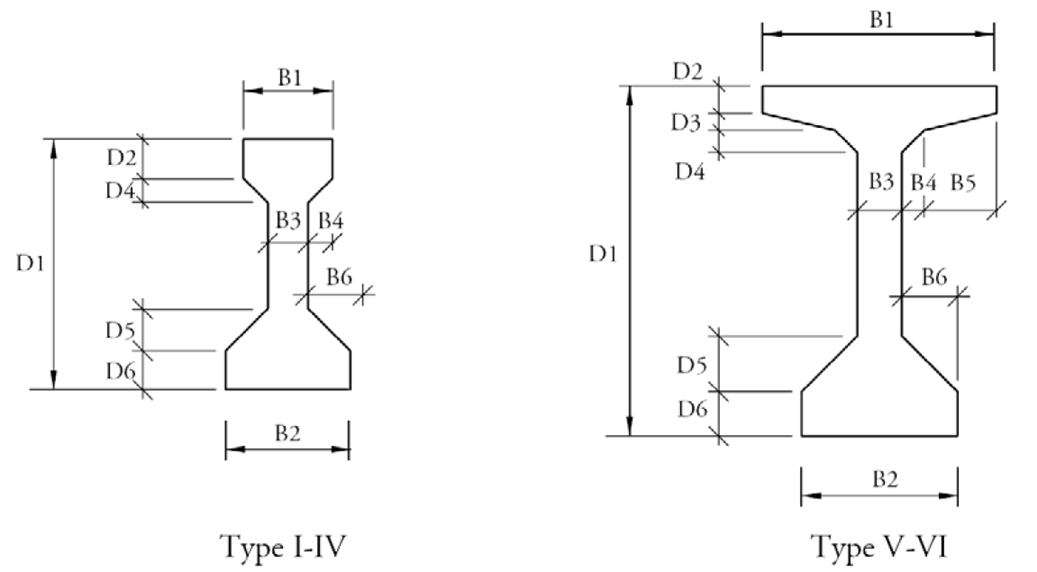
\includegraphics[width=0.5\textwidth]{sectrans_trabes.PNG}
	\label{fig:sectrans_trabes}
	\caption{Sección transversal de trabes AASHTO.}
\end{figure}

Con sus respectivas medidas:

\begin{table}[hbtp!]
\centering
	\label{tab:medidasAASHTO}
	\begin{tabular}{*{7}{c}}
		\rowcolor{BlueGiD!60} Tipo&D1&D2&D3&D4&D5&D6\\
		\rowcolor{BlueGiD!20} I&71&10&0&7.6&13&13\\
		II&91&15&0&7.6&15&15\\
		\rowcolor{BlueGiD!20}III&114&18&0&14&19&18\\
		IV&137&20&0&15&23&20\\
		\rowcolor{BlueGiD!20}V&160&13&7.6&10&25&20\\
		VI&183&13&7.6&10&25&20\\
	\end{tabular}
	\vspace{0.2cm}
	\begin{tabular}{*{7}{c}}
		\rowcolor{BlueGiD!60} Tipo&B1&B2&B3&B4&B5&B6\\
		\rowcolor{BlueGiD!20} I30&41&15&7.6&0&13\\
		II&30&46&15&7.6&0&15\\
		\rowcolor{BlueGiD!20}III&41&56&18&11&0&19\\
		IV&51&66&20&15&0&23\\
		\rowcolor{BlueGiD!20}V&107&71&20&10&33&25\\
		VI&107&71&20&10&33&25\\
	\end{tabular}
	\caption{Medidas de las secciones transversales para las trabes AASHTO (en pulgadas, \textit{in}.}
\end{table}

Lo que necesitamos primero es plantear la estructura del árbol de datos, . Esta podría sintetizarse en el siguiente diagrama:

\begin{figure}[hbt!]\centering
	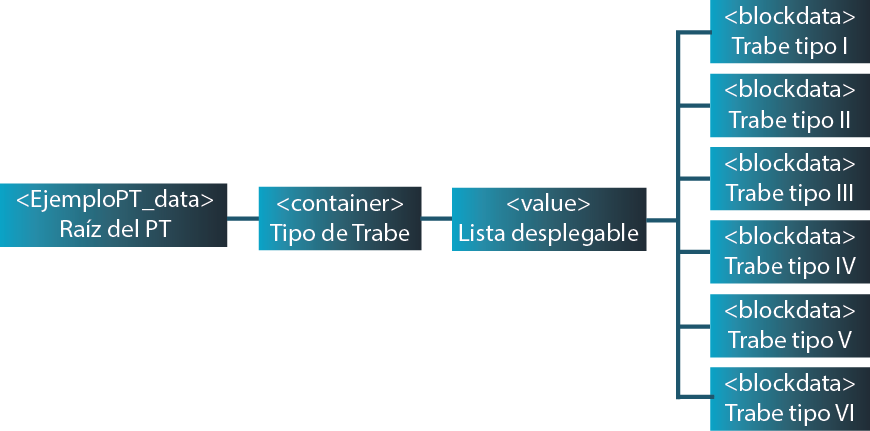
\includegraphics[width=0.45\textwidth]{estructura_spd.PNG}
	\label{fig:estructura_spd}
	\caption{Estructura del archivo SPD de \texttt{EjemploPT.gid}.}
\end{figure}

Lo anterior expone que a partir de la etiqueta/raíz del problem type \texttt{$<$EjemploPT\_data$>$} se crea un \texttt{$<$container$>$} que almacene un cuadro de valores \texttt{$<$value$>$}, este mostrará una lista desplegable con los valores ``Trabe tipo I'', ``Trabe tipo II'', etc., las propiedades geométricas serán almancenadas en las etiquetas \texttt{$<$blockdata$>$}, mismas que fungirán como \textit{base de datos} del problem type.

Organizando la información previa, se detallan los pasos a seguir para el ejemplo:

\begin{enumerate}
	\item Definir los datos de información del problem type en el archivo \texttt{.xml} (Reutilizado de la sección \ref{sec:codigoXML}).
	\item Escribir en el archivo \texttt{.spd} la estructura del árbol de datos tal y como se muestra en la figura \ref{fig:estructura_spd}.
	\item Escribir las rutinas necesarias en el archivo \texttt{.tcl} para cargar el \textit{árbol de datos} e inicializar eñ \texttt{namespace} del problem type.
	\item Crear el catálogo de \texttt{blockdata} que guarde las propiedades geométricas de las trabes (de la tabla \ref{tab:medidasAASHTO}) en un archivo XML. Se puede guardar en al mismo archivo \texttt{.spd} pero aquí lo haré en un archivo separado para mantener una buena práctica de programación.
	\item Hacer una función en TCL que devuelva la lista de los tipos de trabes y vincularla al archivo \texttt{.spd} mediante las etiquetas \texttt{$<$procs$>$}.
	\item Programar un procedimiento en el archivo \texttt{.tcl} que, mediante el tipo de trabe seleccionado en el punto anterior, busque y obtenga las propiedades geométricas almacenadas en el \texttt{blockdata} y las guarde variables globales.
	\item Una vez almacenadas los datos de la geometría, programar el procedimiento en el archivo \texttt{.tcl} para dibujar las trabes de forma paramétrica.
\end{enumerate}


\subsection{Programando el código}

\subsubsection{Archivo \texttt{.spd}}

Una vez escrito el archivo de datos de información del problem type (\texttt{.xml}), escribimos en el archivo \texttt{.spd} en blanco las siguientes líneas de código. El contenido \texttt{CDATA} contiene la llamada de una función que crearemos más adelante llamada \textcolor{blue}{\texttt{EjemploPT::ListaTrabes}}.

\lstset{language=XML} 
\begin{lstlisting}
<?xml version="1.0" encoding="utf-8"?>

<EjemploPT_data version='1.0'>
	<container n="tipoTrabe" pn="Tipo de trabe AASHTO" actualize_tree="1">
		<value n="tipo" pn="Tipo" v="Tipo I" values="[ListaTrabes]" actualize_tree="1"/>
  	</container>
  	<procs>
    	<proc n='ListaTrabes' args='args'>
      	<![CDATA[
        	EjemploPT::ListaTrabes $domNode $args
      	]]>
    	</proc>
  	</procs>
</EjemploPT_data>
\end{lstlisting}

Esto creará una estructura como se deseaba en el la figura \ref{fig:estructura_spd}.

\subsubsection{Archivo \texttt{.tcl}}

Hasta el momento hemos visto cómo crea un \textit{Data tree} (o árbol de datos), pero al cargar nuestro problem type (\texttt{Data$>$Problem type$>$}\textit{Seleccionar problem type de la lista}), la opción para abrirlo no se encuentra por ninguna parte. Esto es porque no hemos escrito nada en el archivo \texttt{.tcl} ni mucho menos \textbf{le hemos especificado al programa que lo abra}. Como se mencionó en secciones previas, el archivo de TCL será aquel que le otorgue la lógica a nuestro programa. Por lo tanto la primera rutina que programaremos será la de abrir el \textit{árbol de datos} inmediatamente cuando carguemos el problem type en GiD, para ello utilizaremos el recurso \texttt{InitGIDProject} visto en la sección \ref{sec:eventosGiD}.

Siguiendo los pasos que se detallan en la sección \ref{sec:consideraciones}, lo que tenemos que hacer es crear un \texttt{namespace} para el problem type, almacenar las variables globales (\texttt{D} y \texttt{B}) que definen la geometría de las trabes e invocar la rutina para abrir el \textit{árbol de datos}. También se creará un submenú para ejecutar el dibujo paramétrico, este se definirá después pero servirá para ejemplificar la creación de menús en TCL. Y por último una serie de rutinas para almacenar la dirección absoluta del problem type (se utilizará después).

\lstset{language=tcl} 
\begin{lstlisting}[caption={Código para inicializar el proyecto y crear el menú.}]
# Proyecto EjemploPT.gid

namespace eval EjemploPT {
	variable D
	variable B
	variable ptDir
}
proc InitGIDProject { dir } {
	EjemploPT::ModificarMenus
	EjemploPT::GuardarDirPT
	gid_groups_conds::open_conditions menu
}
proc EjemploPT::GuardarDirPT { dir } {
	variable ptDir
	set ptDir $dir
}
proc EjemploPT::ObtenerDirPT { } {
	variable ptDir
	return $ptDir
}
proc EjemploPT::ModificarMenus { } {
	GiDMenu::InsertOption "Data" [list "Mostrar Data tree"] 0 PRE [list gid_groups_conds::open_conditions menu] "" "" replace =
	GiDMenu::InsertOption "Data" [list "Mostrar Data tree"] 1 PRE [list EjemploPT::DibujarTrabe] "" "" replace =
    GiDMenu::UpdateMenus
}
\end{lstlisting}

La instrucción \textcolor{blue}{\texttt{gid\_groups\_conds::open\_conditions menu}}, \textcolor{blue}{\texttt{GiDMenu::InsertOption}} y \textcolor{blue}{\texttt{GiDMenu::UpdateMenus}} son rutinas definidas en GiD (definidas en el \textit{Customization Manual}, revisar sintaxis). La primera sirve para leer el archivo \texttt{EjemploPT\_default.spd} y crear una ventana gráfica con los datos leídos, esto es lo que se muestra en el Data Tree. La segunda sirve para agregar submenús en el menú \textit{Data}, agregamos un submenú para abrir el \textit{árbol de datos} (para abrir y cerrarlo) y otro submenú para dibujar (se define esta función más adelante). La tercera, para actualizar los cambios realizados. Si guardamos los cambios en el archivo y ejecutamos el problem type, se abrirá esta ventana:

\begin{figure}[hbt!]\centering
	
\includegraphics[width=0.2\textwidth]{captura_data_tree.PNG}
	\label{fig:estructura_spd}
	\caption{Estructura del archivo \texttt{.spd} vista en el árbol de datos de GiD.}
\end{figure}

Si se ha mostrado la figura anterior, todo se ha cargado con éxito. Pero si se intenta abrir, se generará un error como el que sigue:

\begin{figure}[hbt!]\centering
	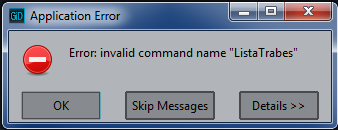
\includegraphics[width=0.35\textwidth]{error_ListaTrabes.PNG}
	\label{fig:error_ListaTrabes}
	\caption{Error cuando GiD no encuentra definida una función.}
\end{figure}

Esto ocurre cuando GiD encuentra la llamada a una función y no la encuentra definida en el archivo TCL. Por ello, la vamos a definir a continuación. Uno de los atributos de la etiqueta \texttt{$<$value$>$} es ``\texttt{values}'' (sección \ref{subsubsec:value}) en la cual transforma el campo de \texttt{value} en lista desplegable si se entrega una cadena de caracteres separados por comas. Entonces la función \textcolor{blue}{\texttt{ListaTrabes}} deberá regresar una lista y se define como sigue (se deberá escribir después de \texttt{InitGIDProject}

\lstset{language=tcl} 
\begin{lstlisting}
proc EjemploPT::ListaTrabes { domNode args } {
	return [list Tipo I , Tipo II , Tipo III , Tipo IV , Tipo V , Tipo VI]
}
\end{lstlisting}

Se guardan los cambios y ahora sí se puede abrir la lista desplegable del \textit{árbol de datos}.

\begin{figure}[hbt!]\centering
	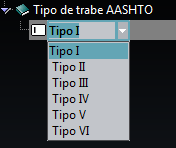
\includegraphics[width=0.25\textwidth]{lista_desplegable.PNG}
	\label{fig:lista_desplegable}
	\caption{Lista desplegable con los tipos de trabes.}
\end{figure}

Ahora se necesita crear la base de datos, para ello se crear una carpeta en el directorio del problem type llamada \texttt{xml} en el directorio del problem type (\texttt{EjemploPT.gid\textbackslash xml}) y almacenamos ahí el archivo (\texttt{basedatostrabes.xml}) donde estará los datos de la geometría (\texttt{blockdata}). El archivo ubicado en \texttt{EjemploPT.gid\textbackslash xml\textbackslash basedatostrabes.xml} quedaría de la siguiente manera:


\lstset{language=XML} 
\begin{lstlisting}[caption={Extracto de la base de datos de la geometría.}]
<?xml version="1.0" encoding="utf-8"?>
<container n="basedatostrabes" pn="Geometria Trabes">
	<blockdata n="seccion" name="Tipo I">
		<value n='d1' pn='D1' v='71'/>
		<value n='d2' pn='D2' v='10'/>
		<value n='d3' pn='D3' v='0'/>
		<value n='d4' pn='D4' v='7.6'/>
		<value n='d5' pn='D5' v='13'/>
		<value n='d6' pn='D6' v='13'/>
		<value n='b1' pn='B1' v='30'/>
		<value n='b2' pn='B2' v='41'/>
... etc
</container>
\end{lstlisting}

Continuando con la escritura del archivo \texttt{.tcl}. Se deben hacer dos cosas:

\begin{itemize}
	\item Obtener el valor del tipo de trabe que seleccione el usuario desde el archivo \texttt{EjemploPT\_default.spd}.
	\item Comparar ese valor con la etiqueta \textcolor{blue}{\texttt{name=}} coincidente de la base de datos y almacenar los datos.
\end{itemize}

La obtención se hace con el paquete \textbf{tdom}, que es un \textit{parser} (\textit{analizador sintáctico}) para XML en TCL, con su respectiva ruta \textbf{XPath}, descritos en secciones posteriores. El paquete se incluirá al principio del código:

\lstset{language=tcl} 
\begin{lstlisting}[caption={Código para inicializar el proyecto y crear el menú.}]
# Proyecto EjemploPT.gid
package require tdom; # Maneja el doc. XML
namespace eval EjemploPT {
	variable D
	variable B
}
...
\end{lstlisting}

Ahora sí definimos la función \texttt{EjemploPT::DibujarTrabe}:

\lstset{language=tcl} 
\begin{lstlisting}[caption={Definición del procedimiento \texttt{EjemploPT::DibujarTrabe}}]
proc EjemploPT::DibujarTrabe { } {
	
	variable D
	variable B
	set D [list ]
	set B [list ]
	set long 500.00
	
	set rootSPD [customlib::GetBaseRoot]
	set tipoTrabe [get_domnode_attribute [$rootSPD selectNodes "\container\[@n='tipoTrabe'\]/value\[@n='tipo'\]"] v]
	
	set XPathBaseDatos [dom parse [tDOM::xmlReadFile [file join [EjemploPT::ObtenerDirPT] "xml/basedatostrabes.xml"]]]
	set domTipoTrabe [$XPathBaseDatos selectNodes "//container\[@n='basedatostrabes'\]"]
	
	foreach domTipoTrabe [$domTipoTrabe childNodes] {
		set strComp [$domTipoTrabe @name]
		if { [string match $tipoTrabe $strComp ] == 1 } {
			set nodoTipo $domTipoTrabe
			break
		}
	}
	
	set D [lappend D [get_domnode_attribute [$nodoTipo selectNodes "value\[@n='d1'\]"] v]]
	set D [lappend D [get_domnode_attribute [$nodoTipo selectNodes "value\[@n='d2'\]"] v]]
	set D [lappend D [get_domnode_attribute [$nodoTipo selectNodes "value\[@n='d3'\]"] v]]
	set D [lappend D [get_domnode_attribute [$nodoTipo selectNodes "value\[@n='d4'\]"] v]]
	set D [lappend D [get_domnode_attribute [$nodoTipo selectNodes "value\[@n='d5'\]"] v]]
	set D [lappend D [get_domnode_attribute [$nodoTipo selectNodes "value\[@n='d6'\]"] v]]
	set B [lappend B [get_domnode_attribute [$nodoTipo selectNodes "value\[@n='b1'\]"] v]]
	set B [lappend B [get_domnode_attribute [$nodoTipo selectNodes "value\[@n='b2'\]"] v]]
	set B [lappend B [get_domnode_attribute [$nodoTipo selectNodes "value\[@n='b3'\]"] v]]
	set B [lappend B [get_domnode_attribute [$nodoTipo selectNodes "value\[@n='b4'\]"] v]]
	set B [lappend B [get_domnode_attribute [$nodoTipo selectNodes "value\[@n='b5'\]"] v]]
	set B [lappend B [get_domnode_attribute [$nodoTipo selectNodes "value\[@n='b6'\]"] v]]
	
	GidUtils::DisableGraphics
	GiD_Process Mescape Geometry Create Line 0.0,0.0 \
											[expr [lindex $B 0]/2.0],0.0 \
											[expr [lindex $B 0]/2.0],[expr -[lindex $D 1]] \
											[expr [lindex $B 2]/2.0],[expr -[lindex $D 1]-[lindex $D 3]] \
											[expr [lindex $B 2]/2.0],[expr -[lindex $D 0]+[lindex $D 4]+[lindex $D 5]] \
											[expr [lindex $B 1]/2.0],[expr -[lindex $D 0]+[lindex $D 4]] \
											[expr [lindex $B 1]/2.0],[expr -[lindex $D 0]] \
											0.0,[expr -[lindex $D 0]] escape
	GiD_Process Mescape Utilities Copy Lines MaintainLayers Mirror FNoJoin 0.0,0.0,0.0 FNoJoin 0.0,1.0,0.0 TwoDim 1 2 3 4 5 6 7 escape
	GiD_Process Mescape Geometry Create NurbsSurface 1 2 3 4 5 6 7 8 9 10 11 12 13 14 escape
	GiD_Process Mescape Utilities Copy Surfaces DoExtrude Volumes MaintainLayers Translation FJoin 1 FNoJoin 0.0,0.0,-500 1 escape
	GiD_Process Mescape Utilities Copy Volumes MaintainLayers MCopy 5 Translation FJoin 1 FNoJoin 60.0,0.0,0.0 1 escape
	GidUtils::EnableGraphics
}
\end{lstlisting}


%----------------------------------------------------------------------------------------
%	BIBLIOGRAPHY
%----------------------------------------------------------------------------------------

\section{Bibliografía}

%\printbibliography[title={Bibliography}] % Print the bibliography, section title in curly brackets

%----------------------------------------------------------------------------------------

\end{document}
